\documentclass[
fontsize=11pt,
paper=a4,
numbers=noenddot
]{scrartcl}

\usepackage[bottom=3cm, top=3cm]{geometry}

\usepackage[utf8]{inputenc}
\usepackage[T1]{fontenc}
\usepackage{microtype}

\usepackage[british]{babel}

\usepackage{subcaption}

\usepackage{booktabs}

\usepackage[backend=biber]{biblatex}
\addbibresource{bibliography.bib}

\usepackage[hidelinks]{hyperref}   

\usepackage{mathtools} 
\usepackage{amsthm}
\usepackage{amssymb}
\usepackage{bm}

\usepackage{tikz}

\newtheorem{theorem}{Theorem}

\usepackage{todonotes}
\usepackage[linesnumbered,ruled,vlined]{algorithm2e}
\SetKwInput{KwData}{Input}

\usepackage{minted}
\usepackage{csquotes}

\addtokomafont{disposition}{\rmfamily}

\title{Parallel Multigrid Monte Carlo\\
{\normalsize Software practical report}}
\date{\small\today}
\author{Nils Friess}

\begin{document}
\maketitle

\begin{abstract}
    This report presents a parallel implementation of the Multigrid Monte Carlo (MGMC) method for sampling from Gaussian random fields on distributed memory machines. 
    %In a certain sense, MGMC is the stochastic counterpart of the classic geometric Multigrid method whereby the smoothers and coarse grid solver are replaced by random Gibbs samplers. 
    We give a brief theoretical introduction to the method before discussing our implementation based on the \emph{Portable and Extensible Toolkit for Scientific computing (PETSc)}. We provide several numerical examples to study the performance and scaling of the parallel implementation.
\end{abstract}

\section{Introduction}
Efficiently generating samples from high-dimensional Gaussian distributions is an important task in many computational sciences but remains computationally challenging when the problem becomes very large
% that the data does not fit in the memory of a single computing node
or when the computation should be sped up by distributing the work among multiple processors. The go--to method for generating Gaussian samples uses a Cholesky factorisation of the covariance matrix or the precision matrix (the inverse covariance matrix) and although the computational cost of the decomposition is $\mathcal{O}(nb^2)$, where $n$ is the number of rows of the covariance/precision matrix and $b$ its bandwidth, it can become prohibitively expensive if the bandwidth is high and cannot be reduced sufficiently using a permutation of the given matrix~\cite{golubvanloan,rue2001fast,foxparker}. Further, the additional memory required to store the Cholesky factor can become problematic for large problems. Iterative methods such as the Gibbs sampler are a popular alternative, but the generated samples are statistically correlated so that in certain situations the cost per \emph{statistically independent} sample can become so large that it renders the method practically useless~\cite{foxparker,kazashimuellerscheichl}. In this report we instead consider the \emph{Multigrid Monte Carlo (MGMC)} method~\cite{goodmansokal} which overcomes the aforementioned limitations. We present a parallel implementation based on the \emph{Portable and Extensible Toolkit for Scientific computing (PETSc)}~\cite{petsc-web-page,petsc-user-ref}.
%It is available as an open-source C++ library under the name \texttt{ParMGMC} available at \url{github.com/nilsfriess/ParMGMC}.

% MGMC scales optimal with respect to the size of the matrix and typically only 2--5 samples are required to obtain a statistically independent sample. 

The report is structured as follows. In the next section we provide a brief introduction to the MGMC method before giving an overview of our parallel implementation in the third section. Since the MGMC method is in a certain sense a stochastic version of the classic (geometric) multigrid algorithm, most components of the algorithm can be parallelised in the same way as in classic multigrid.
% (and are thus already implemented in PETSc, e.g., as part of the \texttt{PCMG} Multigrid preconditioner).
However, certain parts---in particular the parallel Gibbs samplers---have to be implemented from scratch. We will therefore only briefly discuss the parts that are already implemented in PETSc and focus on the  parallelisation of the Gibbs samplers. In the last section we present \textcolor{red}{N} numerical examples to study the parallel performance of our implementation. We conclude with a discussion of open problems and possible research directions.

\section{Multigrid Monte Carlo}
We consider the problem of generating samples from discrete Gaussian random fields with given precision matrix. This includes sampling from Gaussian Markov Random Fields~\cite{rue2005gaussian}, or discretisations of continuous random fields on regular lattices or unstructured grids in $\mathbb{R}^d$, $d=2,3$. Let $\pi\coloneqq\mathcal{N}(A^{-1}f, A^{-1})$ be the target distribution, with $f \in \mathbb{R}^n$ and $A \in \mathbb{R}^{n \times n}$ symmetric positive definite. We assume that $A$ is large but sparse.
%We assume that $A$ is large and sparse which is the case, for instance, if $\pi$ is a \emph[Gaussian Markov random field] (GMRF). 
The standard method to sample from $\pi$ is based on the Cholesky decomposition of $A$. To this end, one computes a Cholesky factorisation $A = LL^T$, with $L \in \mathbb{R}^{n \times n}$ lower triangular, performs the forward-solve $L g = f$, followed by the backward-solve $L^T x = \xi + g$, where $\xi \sim \mathcal{N}(0,I)$. One readily checks that then $x \sim \mathcal{N}(A^{-1}f, A^{-1})$. If $A$ has bandwidth $b$, the cost of generating one sample
% (i.e., the cost of the forward- and backward-solve and of computing the sample $\xi$)
is $\mathcal{O}(2nb)$, and the cost of computing the Cholesky factor is given by $\mathcal{O}(nb^2)$~\cite{golubvanloan}. This is feasible if $b$ is sufficiently small or if a permutation matrix $P$ exists that reduces the bandwidth of $PAP^T$ sufficiently. However, in many practically relevant cases this is not possible, sometimes leading to a computational cost of $\mathcal{O}(n^{7/3})$ to compute the Cholesky factor~\cite{foxparker}.
% \begin{enumerate}
%     \item Draw a sample .
%     \item 
%     \item Backward-solve $L^T x = \xi + g$.
%     \item Return the new sample $x$.
% \end{enumerate}
% Indeed, we then have $x = L^{-T} \xi + L^{-T} g = L^{-T} \xi + {(LL^T)}^{-1} f =  L^{-T} \xi + A^{-1} f$ and by the properties of the normal distribution it follows that $x \sim \mathcal{N}(A^{-1} f, L^{-T}L^{-1}) = \mathcal{N}(A^{-1} f, A^{-1})$ as claimed.

% For large problems, this approach becomes infeasible due to the high cost of the Cholesky factorisation. 

%MGMC was first introduced in the context of simulating lattice field theories as a means to reduce or even eliminate the phenomenon of \emph{critical slowing down}: For classical algorithms, such as the \emph{heat bath} algorithm, the autocorrelation time $\tau$ (the time that is necessary to obtain a new useful grid configuration during the simulation) typically behaves as $\tau \sim h^z$ where $h$ is the grid spacing and usually $z \approx 2$. Thus, as the continuum limit $h \rightarrow 0$ is approached, the computer time increases drastically, rendering these algorithms practically useless. As already described in the original paper~\cite{goodmansokal}, the same holds true when these algorithms are used to generated Gaussian samples (since this simply corresponds to a specific type of Hamiltonian operator that is used to describe the physical theory). In this case, the \emph{heat bath} algorithm is a Gibbs sampler and the autocorrelation time roughly corresponds to the number of samples that need to be generated to obtain one statistically independent sample.

Generalised Gibbs samplers based on matrix splittings~\cite{foxparker} (including the standard Gibbs sampler~\cite{gemangeman}) are popular alternatives in these cases since their computational cost is independent of the bandwidth. Let $A = M - N$ be a matrix splitting with $M$ invertible, and let $y^{(0)} \in \mathbb{R}^n$ be arbitrary. A generalised Gibbs sampler is given by the stochastic iteration
\begin{equation}
    \label{eq:stochasticit}
    M y^{(k+1)} = N y^{(k)} + c^{(k)}\,,\qquad k = 0,1,2, \dotsc,
\end{equation}
with $c^{(k)} \sim \mathcal{N}(f, M^T + N)$. Upon replacing $c^{(k)}$ by $b \in \mathbb{R}^n$ for all $k \in \mathbb{N}_0$, one obtains instead a (deterministic) iterative method for solving the linear system $Ay=b$. By exploiting this similarity, Fox and Parker~\cite{foxparker} have shown that the samples generated by~\eqref{eq:stochasticit} converge in distribution to $\pi$ if, and only if, the corresponding stationary iterative solver converges.
% It is evident that the efficacy of such a sampler depends on the form of $M^T + N$. If $A$ and $M^T + N$ have essentially the same structure, then this approach merely moves the problem of sampling from $\mathcal{N}(0, A)$ to that of sampling from $\mathcal{N}(0, M^T + N)$.

The choice $M = D + L$, $N = -L^T$, where $L$ is the strictly lower triangular part of $A$ and $D$ its diagonal, corresponds to the standard Gibbs sampler, and the deterministic counterpart is the Gauss-Seidel method.
% Using $M = \frac{1}{\omega} D + L$, $N = \frac{1-\omega}{\omega} D - L^T$, for $\omega \in (0,2)$, corresponds to the so called successive over-relaxation Gibbs sampler (or SOR-Gibbs for short). We only consider the standard Gibbs sampler here, which corresponds to $\omega = 1$.
Inserting $M$ and $N$ in~\eqref{eq:stochasticit} gives
\begin{equation*}
    \left(D + L\right) y^{(k+1)} = - L^T y^{(k)} + c^{(k)}\,,
\end{equation*}
with $c^{(k)} \sim \mathcal{N}(f,D)$. Multiplying both sides by $D^{-1}$ and rearranging terms then gives
\begin{equation*}
    y^{(k+1)} = - D^{-1} (L y^{(k+1)} + L^T y^{(k)}) + D^{-1} c^{(k)}\,.
\end{equation*}
Component-wise we thus have
\begin{equation}
    \label{eq:gibbs_comp}
    y^{(k+1)}_j = - \frac{1}{a_{jj}} \left(
      \sum_{m=1}^{j-1} a_{mj} y^{(k+1)}_m + \sum_{m=j+1}^n a_{mj} y^{(k)}_m
    \right) + \frac{1}{a_{jj}} c^{(k)}_j \,,\quad \text{for $j=1,\dotsc,n$.}
\end{equation}
Modifications of the standard Gibbs sampler can be obtained by changing the order in which the components are updated. We call the variant as defined above a forward Gibbs sweep; reversing the order leads to a backward Gibbs sweep. A forward sweep followed by a backward sweep is referred to as a symmetric sweep.  

%Let us first write out the iteration~\eqref{eq:stochasticit}. %Inserting $M$ and $N$ gives
%\begin{equation*}
%    \left(\frac{1}{\omega} D + L\right) y^{(k+1)} = \left(\frac{1-\omega}{\omega} D - L^T\right) y^{(k)} + c^{(k)}\,.
% \end{equation*}
% Multiplying both sides by $\omega D^{-1}$ and rearranging terms then gives
% \begin{equation*}
%     y^{(k+1)} = (1 - \omega) y^{(k)} - \omega D^{-1} (L y^{(k+1)} + L^T y^{(k)}) + \omega D^{-1} c^{(k)}\,.
% \end{equation*}
% Component-wise we have
% \begin{equation*}
%     y^{(k+1)}_j = (1-\omega) y^{(k)}_j - \frac{\omega}{a_{jj}} \left(
%         \sum_{m=1}^{j-1} a_{mj} y^{(k+1)}_m + \sum_{m=j+1}^n a_{mj} y^{(k)}_m
%     \right) + \frac{\omega}{a_{jj}} c^{(k)}_j \,.
% \end{equation*}
% Since the first sum only contains entries of $y^{(k+1)}$ with index \emph{smaller} than $j$, and the second sum only contains entries of $y^{(k)}$ with index \emph{larger} than $j$, one can update the sample in-place, giving Algorithm~\ref{alg:gibbs-sor}. To compute $\omega D^{-1} c^{(k)}$ we first note that since $c^{(k)} \sim \mathcal{N}(f, (2-\omega)/\omega D)$ we have $\omega D^{-1} c^{(k)} \sim \mathcal{N}(\omega D^{-1}f, \omega(2-\omega)D^{-1})$ which we compute by first sampling $z \sim \mathcal{N}(0, I)$ and transforming the result linearly to obtain the correct mean and covariance (see Line 2 of Algorithm~\ref{alg:gibbs-sor}).

If $A$ has $\mathcal{O}(n)$ non-zero entries, the cost of generating one sample using a Gibbs sampler is about $\mathcal{O}(2n)$. However, since the generated samples are highly correlated, multiple iterations are required to obtain one statistically independent sample. If, for instance, $\pi$ is a Gaussian random field discretised on a regular lattice with grid spacing $h$, in certain cases the number of iterations required to obtain a useful sample depends inversely on $h$ so that the computer time increases drastically as $h \rightarrow 0$~\cite{goodmansokal,kazashimuellerscheichl}.
%This behaviour can be explained using the fact that a Gibbs sampler is in a certain sense a stochastic version of the Gauss-Seidel iterative method (see below). It is well-known that the convergence factor of Gauss-Seidel to solve, e.g., a linear system arising from finite difference discretisation of the Poisson equation on a grid, behaves as $1 - \mathcal{O}(h^2)$. 

To overcome this issue, Goodman and Sokal~\cite{goodmansokal} have borrowed ideas from multigrid methods to define a hierarchical sampling algorithm, called \emph{Multigrid Monte Carlo} (MGMC). The general structure is essentially the same as the classic geometric multigrid algorithm~\cite{hackbuschMultiGridMethodsApplications1985}. Suppose we are given a hierarchy of grids. Given a sample on the finest level of the hierarchy, random coarse grid corrections are generated recursively using Gibbs samplers to update the fine grid sample. The Gibbs samplers play the role of the smoothers in classic multigrid and to emphasise the connection, we refer to them as random smoothers in this context. To transfer samples between grids, prolongation and restriction operators are introduced in the same way as in classic  geometric multigrid. If we label the grids from $\ell = 0$ (the coarsest level) to $\ell = L$ (the finest level), and let $n_\ell$ be the number of vertices of grid $\ell$, then we denote by $I_{\ell-1}^\ell \in \mathbb{R}^{n_\ell \times n_{\ell - 1}}$ the so-called \emph{prolongation matrix}. Its transpose $I_{\ell}^{\ell-1} \coloneqq {(I_{\ell-1}^\ell)}^T \in \mathbb{R}^{n_{\ell - 1} \times n_{\ell}}$ is called the \emph{restriction matrix} (for details on how these matrices are defined we refer to the multigrid literature, e.g.,~\cite{hackbuschMultiGridMethodsApplications1985}). Given the fine level precision matrix $A_L \coloneqq A$, the coarse level precision matrices are defined by Galerkin projection
\begin{equation}
  \label{eq:galerkin}
    A_{\ell-1} = I_\ell^{\ell - 1} A_\ell I_{\ell-1}^\ell \in \mathbb{R}^{n_{\ell-1} \times n_{\ell-1}}\,, \quad \text{for\quad$\ell = 1, \dotsc, L$.}
\end{equation}
The matrices $A_\ell$, $\ell = 0, \dotsc, L$, are then used as the precision matrices for the Gibbs samplers on each level. The full MGMC algorithm is summarised in Algorithm~\ref{alg:mgmc}.

\begin{algorithm}
    \DontPrintSemicolon

    \SetKwFunction{Fmgmc}{mgmc}
    \SetKwFunction{Fcoarsesampler}{coarseSampler}
    \SetKwFunction{Frandomsmoother}{randomSmoother}

    \SetKwProg{Fn}{Function}{:}{}

    \SetAlgoLined
    \Fn{\Fmgmc{$y$, $f$, $\ell$}}{
        \If{$\ell == 0$}{
            $y \gets$\Fcoarsesampler{$f$}
        }
        \Else{
            $y \gets$\Frandomsmoother{$A_\ell$, $y$, $f$} \tcp*{Random pre-smoothing}
            $r \gets f - A_\ell y$\tcp*{Compute residual}
            $f^\prime \gets I_{\ell}^{\ell - 1} r$ \tcp*{Restrict residual}
            $v \gets 0$ \tcp*{Initialise coarse grid correction}
            \For{$c =1$ to $\gamma$} {
                $v \gets$ \Fmgmc{$v$, $f^\prime$, $\ell - 1$}
            }
            $y \gets y + I_{\ell-1}^{\ell} v$\tcp*{Prolongate-add the correction}
            $y \gets$\Frandomsmoother{$A_\ell$, $y$, $f$} \tcp*{Random post-smoothing}
        }
        \Return{$y$}
    }

    \caption{Multigrid Monte Carlo}\label{alg:mgmc}
\end{algorithm}

Given a sample $y \in \mathbb{R}^{n_L}$, a new sample $y^\prime \in \mathbb{R}^{n_L}$ is obtained by calling $y^\prime =$ \texttt{mgmc(}$y,\, f,\, L$\texttt{)}. The \emph{cycle parameter} $\gamma$ appearing in line 10 dictates how often the coarser grid is visited. Typically, either $\gamma = 1$ (the so-called V-cycle) or $\gamma = 2$ (the so-called W-cycle) is used. As in classic multigrid, it can be beneficial to run a few iterations of the random smoothers. To keep the presentation simple, this is not included in the algorithm above (but can be configured in our implementation). On the coarsest level one can either use a Gibbs sampler as on the other levels, or a Cholesky sampler (if the coarse problem size is sufficiently small).

As mentioned in the original paper~\cite{goodmansokal} and rigorously proved by Kazashi et al.~\cite{kazashimuellerscheichl} a sequence of samples $y^{(0)}, y^{(1)}, \dotsc$ generated iteratively by 
\begin{equation*}
    y^{(k+1)} = \texttt{mgmc(}y^{(k)},\, f,\, L\texttt{)},\qquad k = 0,1,\dotsc,
\end{equation*}
with $y^{(0)}$ drawn from an arbitrary Gaussian distribution, converges to $\mathcal{N}(A^{-1}f, A^{-1})$ in distribution with a rate that is independent of the grid spacing of the finest level (under suitable conditions). Moreover, the cost of one call to the method is optimal: if the number of smoothing steps, the cycle parameter, and the problems sizes $n_\ell$, $\ell = 0,\dotsc,L$, are chosen suitably, then the cost of one iteration of MGMC is $\mathcal{O}(n_L)$. Lastly, the autocorrelation between the samples is small and also grid-independent.



%This correspondence follows from a general equivalence between stationary iterative methods and so called generalised Gibbs samplers~\cite{foxparker}. In the case of the Gauss-Seidel method, for example, the corresponding sampler is the classical component-wise Gibbs sampler.

%The remaining components of the Multigrid method (in particular, the prolongation and restriction operations) are used in the same way in the MGMC method. An implementation can thus reuse parts of a given Multigrid implementation and for our parallel implementation we can leverage PETSc's optimised parallel implementations of these components. For the coarse sampler, we either use a few iterations of a Gibbs sampler or we generate the samples using a Cholesky factorisation of the coarse matrix. We used the 

\section{\texttt{ParMGMC} -- Parallel Multigrid Monte Carlo}
Having described the general structure of the algorithm, we now discuss our implementation of the MGMC method. We have implemented the algorithm as part of a C++ library called \texttt{ParMGMC} available at \url{github.com/nilsfriess/ParMGMC}.
The library is built on top of the \emph{Portable and Extensible Toolkit for Scientific computing (PETSc)}~\cite{petsc-web-page,petsc-user-ref}, a widely-used software package for the parallel solution of partial differential equations and optimisation problems. PETSc provides a number of parallel data structures and algorithms that are useful for the implementation of the MGMC method. In the following we will go over the individual components of the algorithm and discuss their parallel implementation.

\subsection{Matrices, vectors, parallel communication}
For the parallel distribution and assembly of the matrices and generation of compatible vectors we use PETSc's parallel \texttt{Mat} and \texttt{Vec} formats. Currently, the sequential and parallel variants of the \texttt{MATAIJ} format are supported. Other formats, in particular the \texttt{MATBAIJ} formats, which represent block sparse matrices, are not yet supported. Further, the fact that the precision matrix is necessarily symmetric is not yet exploited to improve performance.

PETSc employs the \emph{Message Passing Interface} (MPI) for parallel communication and provides different abstractions so that direct calls to MPI routines are rarely required. We make use of the \texttt{VecScatter} data structure and associated routines to handle the parallel communication required in the parallel implementation of the Gibbs sampler (see below).

\subsection{Grid hierarchy}
We provide two variants of the MGMC algorithm: the first is based on a grid hierarchy where each grid is implemented using PETSc's \mintinline{cpp}|DMDA| data structure, which is a sub-type of \mintinline{cpp}|DM| (PETSc's abstract base type for grid-like objects), and is used to manage data for a structured grid in up to three dimensions. We provide a class \mintinline{cpp}|DMHierarchy| which has a constructor
\begin{minted}{cpp}
  DMHierarchy(DM coarseSpace, PetscInt nLevels)
\end{minted}
that builds the grid hierarchy using PETSc's \texttt{DMRefine} routine. The constructed \mintinline{cpp}|DMHierarchy| object can then be passed to the constructor of the MGMC sampler together with the precision matrix on the finest level. The constructor has the following signature.
\begin{minted}{cpp}
  MultigridSampler(const std::shared_ptr<LinearOperator> &fineOperator,
                   const DMHierarchy &dmHierarchy,
                   Engine &engine,
                   const MGMCParameters &params)
\end{minted}
The class \mintinline{cpp}|LinearOperator| is a wrapper around PETSc's \mintinline{cpp}|Mat| class that also stores some additional information about the matrix, in particular the colouring (see below).

The parameter \mintinline{cpp}|engine| is a reference to a random number engine. Its type \mintinline{cpp}|Engine| is templated so that different engines can be tested easily. In all instances where random numbers are generated within the class, this engine is used. This ensures that a global random number generator can be defined in the main function and then be passed around so that a single seed is sufficient to determine the randomness of the program.

The last argument can be used to pass additional parameters. The type \mintinline{cpp}|MGMCParameters| has the following structure
\begin{minted}{cpp}
  struct MGMCParameters {
    PetscInt nSmooth;
    MGMCSmoothingType smoothingType;
    MGMCCycleType cycleType;
    MGMCCoarseSamplerType coarseSamplerType;
  };
\end{minted}
The first member variable \mintinline{cpp}|nSmooth| specifies the number of iterations of the random smoothers on each level (the given value is used both for the pre- and the post-smoothers). The next member determines the type of Gibbs sweeps that are performed. Possible values are \mintinline{cpp}|MGMCSmoothingType::ForwardBackward| and \mintinline{cpp}|MGMCSmoothingType::Symmetric|. The first option means that forward sweeps are performed for the pre-smoothers while backward sweeps are performed for the post-smoothers. The second option means that all random smoothers are using symmetric sweeps (i.e., a forward sweep followed by a backward sweep). 

The value of \mintinline{cpp}|cycleType| indicates whether a V-cycle (\mintinline{cpp}|MGMCCycleType::V|) or a W-cycle (\mintinline{cpp}|MGMCCycleType::W|) should be used. The purpose of the last member variable is explained in the next section. 

The second variant of the MGMC sampler allows it to be used with external libraries and more complicated, possibly unstructured grids. In this case, a new sampler class has to be defined which is derived from the \mintinline{cpp}|MultigridSampler| class:
\begin{minted}{cpp}
  template <class Engine> 
  struct ExampleSampler : MultigridSampler<Engine> {
    ExampleSampler(...) : MultigridSampler<Engine>(params, levels, engine) {
      ...
      for (int l = 0; l < levels; ++l)
        this->ops[l] = std::make_shared<parmgmc::LinearOperator>(...);
      ...
    }

    PetscErrorCode restrict(std::size_t level, Vec residual, 
                            Vec f) override { ... }

    PetscErrorCode prolongateAdd(std::size_t level, Vec coarse,
                                 Vec fine) override { ... }
  };    
\end{minted}
The constructor of this new class has to call the constructor of the base class with the desired parameters, the number of levels and the random number engine. It must also define the operators for each level as depicted in the for loop. Further, since there is no \texttt{DMHierarchy} any more, the class has to override the methods \texttt{restrict} and \mintinline{cpp}|prolongateAdd| which correspond to lines 8 and 13 of Algorithm~\ref{alg:mgmc}, respectively.

\subsection{Coarse grid sampler}
The original paper~\cite{goodmansokal} uses Gibbs samplers on all grids, including the coarsest. As in classic multigrid, it is also possible to use a direct method on the coarsest grid (if the problem size there is sufficiently small). We have implemented both approaches, selectable via the the \mintinline{cpp}|MGMCCoarseSamplerType| parameter in the \mintinline{cpp}|MGMCParameters| class (see above). Possible values are \mintinline{cpp}|MGMCCoarseSamplerType::Standard| (which uses to $2 \times \texttt{nSmooth}$ symmetric Gibbs sweeps on the coarsest level) and \mintinline{cpp}|MGMCCoarseSamplerType::Cholesky|.

 In the case where a Cholesky sampler is used on the coarsest level, we rely on the PARDISO implementation of the Intel Math Kernel Library (MKL)~\cite{intelmkl} which provides both a serial and a parallel implementation of sparse Cholesky factorisation and the possibility to perform the forward substitution and the backward substitution step separately (we found that most other parallel Cholesky implementations lack this option). We access the Intel MKL library through an abstraction layer provided by PETSc.\footnote{At the time of writing, not all options of the Intel MKL PARDISO implementation are accessible from PETSc. The option to perform the forward and backward substitutions individually was only recently contributed to PETSc by the author and is not yet included in a released PETSc version.} 

\subsection{Gibbs samplers (random smoothers)}
%Before discussing the parallelisation of the Gibbs samplers on distributed memory machines, let us first discuss the serial implementation of the Gibbs sampler in more detail. We only consider the standard Gibbs sampler here but everything readily extends to SOR-Gibbs.

% As briefly discussed in the previous section, the standard Gibbs sampler is given by the stochastic iteration~\eqref{eq:stochasticit} with $M = D + L$ and $N = -L^T$. Inserting $M$ and $N$ gives
% \begin{equation*}
%     \left(D + L\right) y^{(k+1)} = - L^T y^{(k)} + c^{(k)}\,,
% \end{equation*}
% with $c^{(k)} \sim \mathcal{N}(f,D)$. Multiplying both sides by $D^{-1}$ and rearranging terms then gives
% \begin{equation*}
%     y^{(k+1)} = - D^{-1} (L y^{(k+1)} + L^T y^{(k)}) + D^{-1} c^{(k)}\,.
% \end{equation*}
Recall the component-wise form of the Gibbs sweep
\begin{equation}
    y^{(k+1)}_j = - \frac{1}{a_{jj}} \left(
        \sum_{m=1}^{j-1} a_{mj} y^{(k+1)}_m + \sum_{m=j+1}^n a_{mj} y^{(k)}_m
      \right) + \frac{1}{a_{jj}} c^{(k)}_j \,,\quad \text{for $j=1,\dotsc,n$.}
      \label{eq:gibbs_comp2}
\end{equation}
%Since the second sum only contains entries of the previous sample $y^{(k)}$ with index \emph{larger} than $j$, one can update the sample in-place. 
%To compute $D^{-1} c^{(k)}$ first note that since $c^{(k)} \sim \mathcal{N}(f, D)$ it holds that $D^{-1} c^{(k)} \sim \mathcal{N}(D^{-1}f, D^{-1})$ which can be computed by first sampling $z \sim \mathcal{N}(0, I)$ and transforming the result as $D^{-1/2}z + D^{-1}f$.

To parallelise~\eqref{eq:gibbs_comp}, we exploit to sparse structure of $A$. Let us first consider a simple example and then extend the idea below. Consider the grid in Fig.~\ref{fig:lattice1} and define the precision matrix $A \in \mathbb{R}^{25 \times 25}$ as
\begin{equation*}
   a_{ij} = 
   10^{-4} \delta_{ij} + 
    \begin{cases}
        4 & \text{if $i = j$,} \\
        -1 &  \text{if $i \neq j$ and vertex $i$ and vertex $j$ are neighbours,} \\
        0 & \text{otherwise,}
    \end{cases}
\end{equation*} 
%The second condition is true if the vertices $i$ and $j$ are connected by an edge in the graph, and $n_i$ is the number of neighbours of node $i$ (i.e., the number of edges connected to it). Note that the non-zero structure of $A$ is the same as that of a standard five-point stencil finite difference discretisation of the Laplacian on the grid.
Let $y^{(k)}$ be a sample on the grid, flattened into a vector in $\mathbb{R}^{25}$. The key observation is that one can change the order in which the components in~\eqref{eq:gibbs_comp2} are updated and partition the indices into two sets such that the components within the sets can be updated in parallel. Consider for instance the grid point $7$ in Fig.~\ref{fig:lattice1}. To update its value only the value of its direct neighbours is required due to the local structure of the precision matrix. Collecting all vertices that can be updated independently of each other in separate sets, one obtains a vertex colouring of the graph. In this case, two colours (traditionally, red and black) are sufficient as depicted in Fig.~\ref{fig:lattice2}.

\begin{figure}[htpb]
    \centering
    \begin{subfigure}[t]{.48\linewidth}
        \centering
        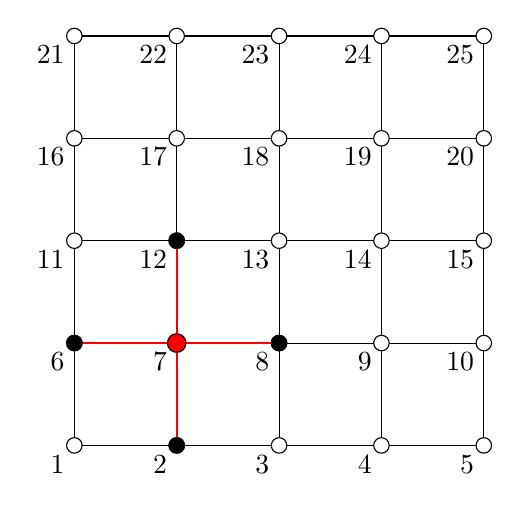
\begin{tikzpicture}[scale=1.3]
            \draw (0,0) grid (4,4);

            \foreach \x in {0,...,4}{
                \foreach \y in {0,...,4}{
                    \pgfmathsetmacro\result{int(5 * \y + \x + 1)}
                    \draw[fill=white] (\x,\y) circle (.5ex);
                    \draw (\x,\y) node[anchor=north east] {$\result$};
                }
            }
            
            \draw[thick,red] (1,1) -- +(0,1);
            \draw[thick,red] (1,1) -- +(1,0);
            \draw[thick,red] (1,1) -- +(-1,0);
            \draw[thick,red] (1,1) -- +(0,-1);
            
            \draw[fill=red] (1,1) circle (0.6ex);

            \draw[fill=black] (1,1)+(0,1) circle (0.5ex);
            \draw[fill=black] (1,1)+(1,0) circle (0.5ex);
            \draw[fill=black] (1,1)+(0,-1) circle (0.5ex);
            \draw[fill=black] (1,1)+(-1,0) circle (0.5ex);
        \end{tikzpicture}
        \caption{The node with index $7$ only depends on its direct neighbours.}\label{fig:lattice1}
    \end{subfigure}\hfill%
    \begin{subfigure}[t]{.48\linewidth}
        \centering
        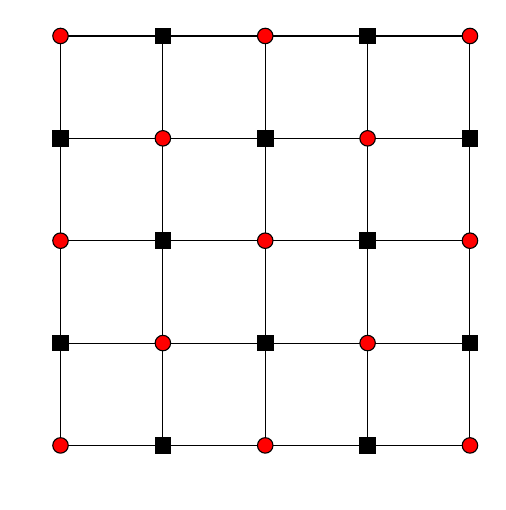
\begin{tikzpicture}[scale=1.3]
            \draw (0,0) grid (4,4);
            \draw[fill=red] (0,0) circle (.5ex);
            \draw[fill=red] (0,2) circle (.5ex);
            \draw[fill=red] (0,4) circle (.5ex);
            \draw[fill=red] (1,1) circle (.5ex);
            \draw[fill=red] (1,3) circle (.5ex);
            \draw[fill=red] (2,0) circle (.5ex);
            \draw[fill=red] (2,2) circle (.5ex);
            \draw[fill=red] (2,4) circle (.5ex);
            \draw[fill=red] (3,1) circle (.5ex);
            \draw[fill=red] (3,3) circle (.5ex);
            \draw[fill=red] (4,0) circle (.5ex);
            \draw[fill=red] (4,2) circle (.5ex);
            \draw[fill=red] (4,4) circle (.5ex);

            \newcommand\Square[1]{+(-#1,-#1) rectangle +(#1,#1)}
            \draw[fill=black] (0,1) \Square{0.5ex};
            \draw[fill=black] (0,3) \Square{0.5ex};
            \draw[fill=black] (1,0) \Square{0.5ex};
            \draw[fill=black] (1,2) \Square{0.5ex};
            \draw[fill=black] (1,4) \Square{0.5ex};
            \draw[fill=black] (2,1) \Square{0.5ex};
            \draw[fill=black] (2,3) \Square{0.5ex};
            \draw[fill=black] (3,0) \Square{0.5ex};
            \draw[fill=black] (3,2) \Square{0.5ex};
            \draw[fill=black] (3,4) \Square{0.5ex};
            \draw[fill=black] (4,1) \Square{0.5ex};
            \draw[fill=black] (4,3) \Square{0.5ex};

            \draw (0,0) node[anchor=north east] {\phantom{$1$}};
        \end{tikzpicture}
        \caption{Extending the idea creates a red/black colouring of the lattice.}\label{fig:lattice2}
    \end{subfigure}
    \caption{A two-dimensional $5 \times 5$ lattice.}\label{fig:lattice}
  \end{figure}
  
%This allows to first update all red nodes in parallel, and then all black nodes in parallel, resulting in the red/black Gibbs sampler.
%We provide a method \mintinline{cpp}|colorMatrix(DM)| in the class \mintinline{cpp}|LinearOperator| which creates a red/black colouring for the given \mintinline{cpp}|DM| and the Gibbs sampler (defined by the class \mintinline{cpp}|MulticolorGibbsSampler|) will then use this colouring.

If the data dependencies between nodes are more complex (e.g., when the local neighbourhood that influences a node is bigger, or when the problem is not posed on a simple grid but an unstructured mesh), more colours will be necessary to colour the nodes such that no two nodes of the same colour depend on each other. Note that due to~\eqref{eq:galerkin}, the number of colours that are necessary to colour the graph of a coarse level matrix $A_{\ell-1}$ can generally be bigger than the number of colours required for $A_{\ell}$.
%In this case the method \mintinline{cpp}|LinearOperator::colorMatrix()| can be called without any arguments, in which case PETSc's matrix colouring routines will be called to partition the indices appropriately. These functions directly operate on the matrix graph and therefore do not need any information about the underlying geometry of the problem.

This allows to parallelise the method in a shared-memory context. If the problem is scattered on different processes that do not share common memory, communication between the processes is necessary. Suppose the grid is distributed among four processes as depicted in Fig.~\ref{fig:latticedist} (we labelled the vertices using PETSc's standard ordering). A distributed-memory parallel Gibbs sampler can then be defined as follows:
\begin{enumerate}
    \item Send/receive values at the black boundary vertices.
    \item Perform the Gibbs sweep defined by~\eqref{eq:gibbs_comp} for the red vertices.
    \item Send/receive values at the red boundary vertices.
    \item Perform the Gibbs sweep defined by~\eqref{eq:gibbs_comp} for the black vertices.
\end{enumerate}
The extension to colourings with more than two colours is straightforward: First send/receive the values that the nodes of the current colour depend on, then update those nodes, and proceed with the next colour.

\begin{figure}[htpb]
    \centering
    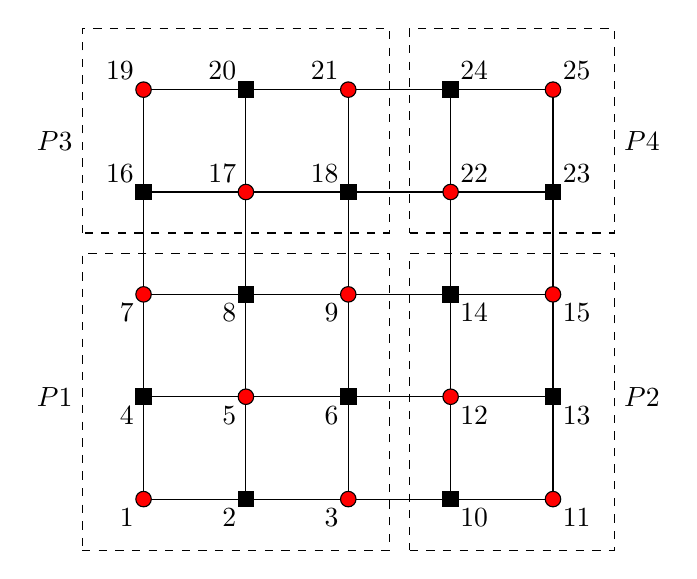
\begin{tikzpicture}[scale=1.3]
        \draw (0,0) grid (4,4);
        \draw[fill=red] (0,0) circle (.5ex);
        \draw[fill=red] (0,2) circle (.5ex);
        \draw[fill=red] (0,4) circle (.5ex);
        \draw[fill=red] (1,1) circle (.5ex);
        \draw[fill=red] (1,3) circle (.5ex);
        \draw[fill=red] (2,0) circle (.5ex);
        \draw[fill=red] (2,2) circle (.5ex);
        \draw[fill=red] (2,4) circle (.5ex);
        \draw[fill=red] (3,1) circle (.5ex);
        \draw[fill=red] (3,3) circle (.5ex);
        \draw[fill=red] (4,0) circle (.5ex);
        \draw[fill=red] (4,2) circle (.5ex);
        \draw[fill=red] (4,4) circle (.5ex);

        \newcommand\Square[1]{+(-#1,-#1) rectangle +(#1,#1)}
        \draw[fill=black] (0,1) \Square{0.5ex};
        \draw[fill=black] (0,3) \Square{0.5ex};
        \draw[fill=black] (1,0) \Square{0.5ex};
        \draw[fill=black] (1,2) \Square{0.5ex};
        \draw[fill=black] (1,4) \Square{0.5ex};
        \draw[fill=black] (2,1) \Square{0.5ex};
        \draw[fill=black] (2,3) \Square{0.5ex};
        \draw[fill=black] (3,0) \Square{0.5ex};
        \draw[fill=black] (3,2) \Square{0.5ex};
        \draw[fill=black] (3,4) \Square{0.5ex};
        \draw[fill=black] (4,1) \Square{0.5ex};
        \draw[fill=black] (4,3) \Square{0.5ex};

        \draw[dashed] (-0.6,-0.5) -- (2.4, -0.5) -- (2.4,2.4) -- (-0.6,2.4) -- cycle;
        \draw[dashed] (2.6,-0.5) -- (4.6, -0.5) -- (4.6,2.4) -- (2.6,2.4) -- cycle;
        \draw[dashed] (-0.6,2.6) -- (-0.6, 4.6) -- (2.4,4.6) -- (2.4,2.6) -- cycle;
        \draw[dashed] (2.6,2.6) -- (4.6, 2.6) -- (4.6,4.6) -- (2.6,4.6) -- cycle;

        \draw (-0.6, 1) node[anchor=east] {$P1$};
        \draw (4.6, 1) node[anchor=west] {$P2$};
        \draw (-0.6, 3.5) node[anchor=east] {$P3$};
        \draw (4.6, 3.5) node[anchor=west] {$P4$};

        \draw (0,0) node[anchor=north east] {$1$};
        \draw (1,0) node[anchor=north east] {$2$};
        \draw (2,0) node[anchor=north east] {$3$};
        \draw (0,1) node[anchor=north east] {$4$};
        \draw (1,1) node[anchor=north east] {$5$};
        \draw (2,1) node[anchor=north east] {$6$};
        \draw (0,2) node[anchor=north east] {$7$};
        \draw (1,2) node[anchor=north east] {$8$};
        \draw (2,2) node[anchor=north east] {$9$};

        \draw (3,0) node[anchor=north west] {${10}$};
        \draw (4,0) node[anchor=north west] {${11}$};
        \draw (3,1) node[anchor=north west] {${12}$};
        \draw (4,1) node[anchor=north west] {${13}$};
        \draw (3,2) node[anchor=north west] {${14}$};
        \draw (4,2) node[anchor=north west] {${15}$};

        \draw (0,3) node[anchor=south east] {${16}$};
        \draw (1,3) node[anchor=south east] {${17}$};
        \draw (2,3) node[anchor=south east] {${18}$};
        \draw (0,4) node[anchor=south east] {${19}$};
        \draw (1,4) node[anchor=south east] {${20}$};
        \draw (2,4) node[anchor=south east] {${21}$};

        \draw (3,3) node[anchor=south west] {${22}$};
        \draw (4,3) node[anchor=south west] {${23}$};
        \draw (3,4) node[anchor=south west] {${24}$};
        \draw (4,4) node[anchor=south west] {${25}$};
    \end{tikzpicture}
    \caption{The two-dimensional lattice distributed on four processes using PETSc's default global indexing scheme.}\label{fig:latticedist}
\end{figure}

%If we consider process $P1$, for instance, it would first send the values at index $6$ to $P2$ and the value at index $8$ to $P3$. It would then receive values at indices $10, 14, 16$ and $18$ from $P2$ and $P3$, respectively. Then it updates its red inidices before sending the updated values at indices $3, 7$ and $9$, and receiving the updated values for the vertices $12$ and $17$. Lastly, it updates its black vertices. 

The actual colouring of the matrix is handled in the \texttt{LinearOperator} class which provides a method \texttt{colorMatrix()} (which generates a general colouring using PETSc's \texttt{MatColoring} routines), and an overloaded variant \texttt{colorMatrix(DM)} which generates a red/black colouring compatible with the given \texttt{DM}.

As mentioned above, we use PETSc's \mintinline{cpp}|VecScatter| data structures to handle the parallel communication. For each colour, a \mintinline{cpp}|VecScatter| context is defined and the send/receive steps above are then implemented as
\begin{minted}{cpp}
  auto scatter = linearOperator->getColoring()->getScatter(i);
  auto ghostvec = linearOperator->getColoring()->getGhostVec(i);

  VecScatterBegin(scatter, sample, ghostvec, 
                  INSERT_VALUES, SCATTER_FORWARD);
  VecScatterEnd(scatter, sample, ghostvec, 
                INSERT_VALUES, SCATTER_FORWARD);
\end{minted}
This scatters the values of \mintinline{cpp}|sample| at boundary nodes on remote processes into the vector \mintinline{cpp}|ghostVec| that is then used during the Gibbs sweep. 
%PETSc also has the concept of \emph{local vectors} (as opposed to \emph{global vectors}) on that include the so-called ghost indices (i.e., for the grid in Fig.~\ref{fig:latticedist} a local vector on process $P1$ would not only contain its local indices $1$--$9$ but also the remote indices $10,12,14,16,17$ and $18$), and provides functions that handle the scattering of the ghost values automatically. However, since we repeatedly need access only to portions of the remote boundary nodes (namely the ones of the same colour), and we want the Gibbs sampler to be independent of the underlying geometry and only require access to the precision matrix itself, we instead decided to work with the low-level \mintinline{cpp}|VecScatter| structures directly.

A multicolouring approach is not the only option to parallelise a Gibbs sampler. Due to the structural similarity of the Gibbs sampler to the Gauss-Seidel method, parallelisation strategies for Gauss-Seidel methods can directly be applied to a parallel Gibbs sampler implementation. One approach that works directly on the level of the matrix graph is presented in~\cite{adams2001}, and it is demonstrated that it outperforms multicolour Gauss-Seidel in cases where many colours are necessary to partition the nodes appropriately. Instead of colouring the vertices, the algorithm first introduces an ordering between the processes. Then, boundary nodes are partitioned into three sets: the \emph{top} nodes (which only communicate with lower processes), the \emph{bot} nodes (which only communicate with higher processes), and the \emph{mid} nodes (the remaining boundary nodes). The algorithm then proceeds by first updating top, then mid, then bot nodes. Parallel communication of the updated nodes is overlapped with the computation for the interior nodes, and only when updating the mid nodes it might be necessary to wait for other processes to finish first. We have not implemented this method yet, but plan to do so in a future version.

Other parallelisation strategies for Gauss-Seidel exploit that it is typically not used as a standalone solver but only as a smoother in multigrid. In this case, local Gauss-Seidel sweeps are performed independently on each process, communicating boundary values only after each full sweep (i.e., data dependencies between nodes across processor boundaries are ignored during the sweeps). When used as a solver, this approach might not converge to the correct solution but it often works sufficiently well when used as a multigrid smoother~\cite{parmultigrid}. The equivalent Gibbs sampler, usually referred to as \emph{Hogwild} Gibbs~\cite{hogwild}, has also been studied in the literature, although the generated samples do not converge to the target distribution. Our library also provides a class \mintinline{cpp}|HogwildGibbsSampler| which implements this sampler using PETSc's parallel Gauss-Seidel implementation. We use this sampler in our numerical experiments as a baseline to measure the overhead of the parallel communication due to the colouring.

%To define the MGMC sampler as an analogue of the Multigrid method, Goodman and Sokal~\cite{goodmansokal} exploited a close connection between the Gauss-Seidel iterative method and the Gibbs sampler. Fox and Parker showed that this connection is only a special case of a broader correspondence between iterative methods based on matrix splittings and so called generalised Gibbs samplers.

%Recall that the target distribution is $\pi \coloneqq \mathcal{N}(A^{-1}f, A^{-1})$ with $(A, f) \in \mathbb{R}^{n \times n} \times \mathbb{R}^n$ and $A$ symmetric positive definite. Let now $A = M - N$ be a matrix splitting with $M$ invertible, and let $y^{(0)} \in \mathbb{R}^n$ be arbitrary. Then, the stochastic iteration
%\begin{equation}
%    \label{eq:stochasticit}
%    M y^{(k+1)} = N y^{(k)} + c^{(k)}\,,\qquad k = 0,1,2, \dotsc,
%\end{equation}
%with $c^{(k)} \sim \mathcal{N}(f, M^T + N)$, converges in distribution to $\pi$ (see~\cite[Thm.\ 2 and Cor.\ 4]{foxparker}). It is evident that the practicality of a sampler derived from this idea depends on the form of $M^T + N$. If $A$ and $M^T + N$ have essentially the same structure, then this approach merely moves the problem of sampling from $\mathcal{N}(0, A)$ to that of sampling from $\mathcal{N}(0, M^T + N)$. It turns out that the choice $M = D + L$, $N = -L^T$ lies at a sweet spot since $M^T + N = D$ and thus sampling from $\mathcal{N}(f, M^T + N)$ is easy, and solving the linear system in~\eqref{eq:stochasticit} is also simple (see below). Here, $L$ is the strictly lower triangular part of $A$ and $D$ is the diagonal. In the deterministic case, this matrix splitting defines a Gauss-Seidel solver; in the stochastic case, this is a Gibbs sampler. Using $M = \frac{1}{\omega} D + L$, $N = \frac{1-\omega}{\omega} D - L^T$, for $\omega \in (0,2)$, offers the same advantages and corresponds to the method of successive over-relaxation (SOR) in the deterministic case and we refer to the stochastic variant as SOR-Gibbs. Since this reduces to a standard Gibbs sampler for $\omega = 1$, we now study SOR-Gibbs in detail.


%\begin{equation*}
%    \left(\frac{1}{\omega} D + L\right) y^{(k+1)} = \left(\frac{1-\omega}{\omega} D - L^T\right) y^{(k)} + c^{(k)}\,.
% \end{equation*}
% Multiplying both sides by $\omega D^{-1}$ and rearranging terms then gives
% \begin{equation*}
%     y^{(k+1)} = (1 - \omega) y^{(k)} - \omega D^{-1} (L y^{(k+1)} + L^T y^{(k)}) + \omega D^{-1} c^{(k)}\,.
% \end{equation*}
% Component-wise we have
% \begin{equation*}
%     y^{(k+1)}_j = (1-\omega) y^{(k)}_j - \frac{\omega}{a_{jj}} \left(
%         \sum_{m=1}^{j-1} a_{mj} y^{(k+1)}_m + \sum_{m=j+1}^n a_{mj} y^{(k)}_m
%     \right) + \frac{\omega}{a_{jj}} c^{(k)}_j \,.
% \end{equation*}
% Since the first sum only contains entries of $y^{(k+1)}$ with index \emph{smaller} than $j$, and the second sum only contains entries of $y^{(k)}$ with index \emph{larger} than $j$, one can update the sample in-place, giving Algorithm~\ref{alg:gibbs-sor}. To compute $\omega D^{-1} c^{(k)}$ we first note that since $c^{(k)} \sim \mathcal{N}(f, (2-\omega)/\omega D)$ we have $\omega D^{-1} c^{(k)} \sim \mathcal{N}(\omega D^{-1}f, \omega(2-\omega)D^{-1})$ which we compute by first sampling $z \sim \mathcal{N}(0, I)$ and transforming the result linearly to obtain the correct mean and covariance (see Line 2 of Algorithm~\ref{alg:gibbs-sor}).

% \begin{algorithm}[htpb]
%     \SetAlgoLined
%     \KwData{Precision matrix $A$, vector $f$, SOR parameter $\omega$, number of iterations $K$, initial sample $y$}
%     \KwResult{Sample $y$}
%     \For{$k \leftarrow 1$ \KwTo $K$}{
%       Sample $z \sim \mathcal{N}(0, I)$ \;
%       Transform $z \leftarrow \sqrt{\omega(2 - \omega)} D^{-1/2} z + \omega D^{-1} f$ \;
%       Update $y_j \leftarrow (1-\omega) y_j - \frac{\omega}{a_{jj}} \left(
%             \sum_{m=1}^{j-1} a_{mj} y_m + \sum_{m=j+1}^n a_{mj} y_m
%         \right) + z$ \;
%     }
%     \caption{SOR-Gibbs sampler}\label{alg:gibbs-sor}
%   \end{algorithm}


\section{Numerical results}\label{sec:numerics}
In this section we study the performance of our implementation.
%Here we only consider the parallel scalability and the overhead caused by colouring. We leave a comparison with other state of the art sampling algorithms for future work.
Let us begin with a description of the random field. The precision matrix is a discretisation (using either finite differences or finite elements, see below) of a shifted Laplace operator
\begin{equation}
    \label{eq:shiftedlaplace}
    \mathcal{A} u \coloneqq (\kappa^2 - \Delta) u \qquad \text{for some } \kappa > 0 \,.
\end{equation}
The reason for this specific choice of precision operator is due to a result by Whittle~\cite{whittle1954,whittle1963} (see also~\cite{lindgren,lindgrenSPDEApproachGaussian2022}). Consider the stochastic partial differential equation (SPDE) $\tau (\kappa^2 - \Delta)^{\alpha/2} u = \mathcal{W}$, where $\tau$ is a normalisation parameter that we ignore in the following, and $\mathcal{W}$ is spatial white noise. The stationary solutions of this SPDE have Mat\'ern covariance function with smoothness parameter $\nu = \alpha - d/2$ where $d$ is the dimension of the domain. The associated precision operator is $\mathcal{A} \coloneqq {(\kappa^2 - \Delta)}^\alpha$~\cite[Sec.\ 2.2]{lindgrenSPDEApproachGaussian2022}, and we see that~\eqref{eq:shiftedlaplace} corresponds to $\alpha = 1$. The smoothness parameters of the associated Mat\'ern fields are then $\nu = 0$ in 2D and $\nu = -\frac{1}{2}$ in 3D, respectively.

We consider two variants that differ in the way~\eqref{eq:shiftedlaplace} is discretised on the finest level to obtain the precision matrix $A_L$. In the first, the operator~\eqref{eq:shiftedlaplace} is discretised on the unit square ${[0,1]}^2$ using a five-point finite difference stencil. In the second, we instead discretise~\eqref{eq:shiftedlaplace} on two unstructured grids using $H^1$ conforming finite elements using the MFEM library~\cite{mfem,mfem-web}. Both cases use homogenous Dirichlet boundary conditions. The mean $f$ is set to zero. All examples use MGMC configured to run a V-cycle and use two iterations of the random smoothers.
% We measure the time to set up the samplers and to generate a fixed number of samples, and study how the execution time changes with increasing nunber of processors. We either fix the total problem size (strong scaling) or we fix the local per-processor problem size (weak scaling).

% For each problem we carry out the following experiments. We compare the performance of the multicolour Gibbs sampler to the Hogwild Gibbs sampler to study the overhead due to the colouring. Further, we study the strong scaling (i.e., the global problem size is fixed) and weak scaling (i.e., the problem size per processor is fixed) on up to 2048 cores of the multicolour Gibbs sampler, the Hogwild Gibbs sampler, and the MGMC sampler (both with multicolour Gibbs and Hogwild Gibbs as random smoothers). In all cases, we measured the time to set up the samplers and the time to sample a fixed number of samples. When testing the Gibbs samplers stand-alone, we have always executed the tests using the finest grid in the hierarchy.

The purpose of the following examples is not to study the statistical properties of the samples generated by MGMC or to compare the performance to other state-of-the-art samplers. Here we focus on the parallel performance of our implementation with particular regard to the overhead caused by the colouring. We also compare the runtime and scalability of using a Cholesky sampler on the coarsest grid and the variant that uses Gibbs samplers on all levels.

\subsection{Structured grid}
We begin with a study of the strong scaling behaviour. To this end, we set up a grid hierarchy with five levels, the coarsest level being of size $257 \times 257$ and the finest level consisting of $4097 \times 4097$ grid points. Since we use a simple 5-point finite difference stencil to discretise~\eqref{eq:shiftedlaplace}, two colours are sufficient to colour the lattice on the finest level. On the remaining levels, the colouring routines implemented in PETSc produced colourings with nine ($\ell = 3$), eight ($\ell = 2$), eight ($\ell = 1$), and nine colours ($\ell = 0$), respectively.

\begin{figure}[htpb]
    \centering
    \begin{subfigure}[b]{0.49\textwidth}
        \centering
        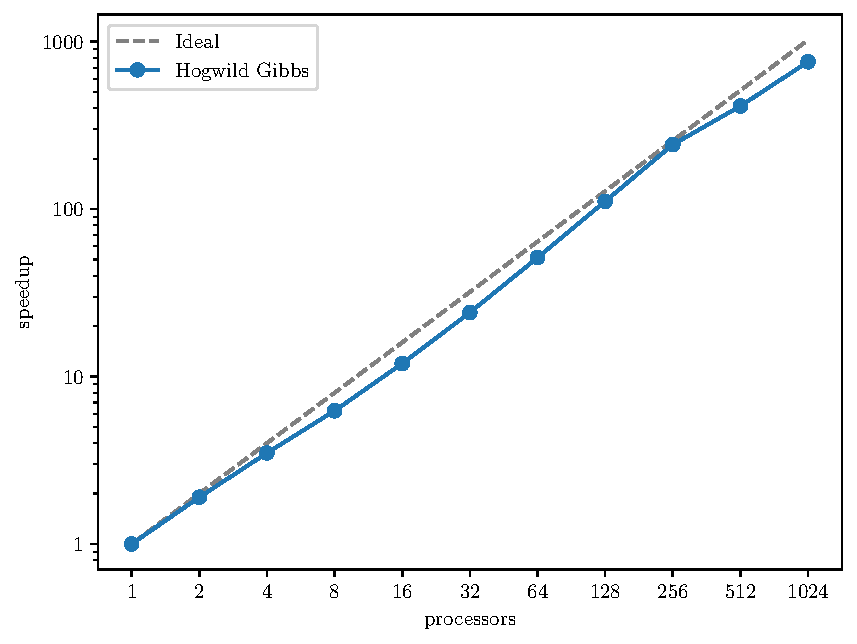
\includegraphics[width=\textwidth]{plots/strong_scaling_hogwild_4097x4097.pdf}
    \end{subfigure}
    \hfill
    \begin{subfigure}[b]{0.49\textwidth}
        \centering
        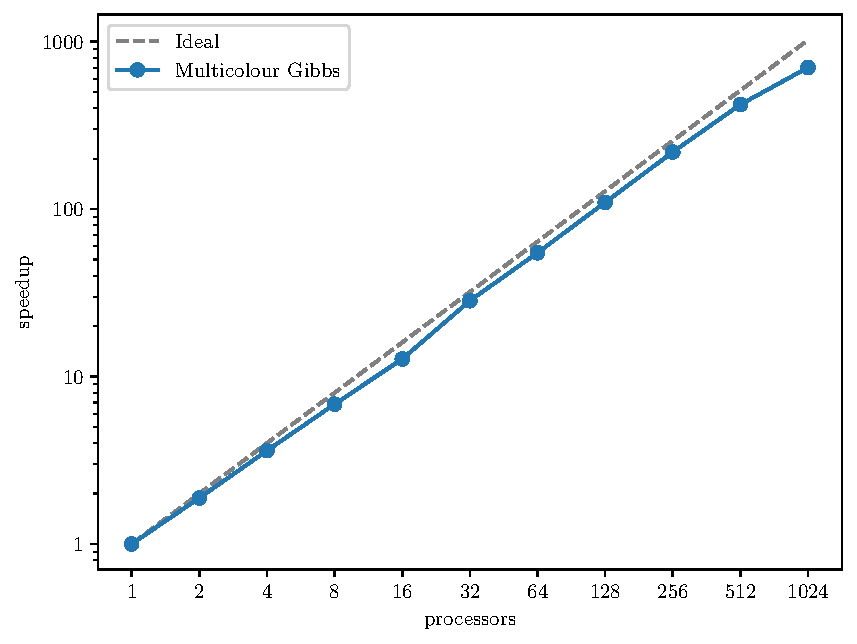
\includegraphics[width=\textwidth]{plots/strong_scaling_gibbs_4097x4097.pdf}
      \end{subfigure}
      \caption{Strong scaling speed-up for the Hogwild Gibbs sampler (left) and the multicolour Gibbs sampler (right). The multicolour Gibbs sampler uses two colours in this case.}
    \label{fig:2d_structured_ss}
\end{figure}

We begin with a comparison of the Hogwild Gibbs sampler and the multicolour Gibbs sampler used as standalone samplers on the finest level. In Fig.~\ref{fig:2d_structured_ss} we plot the strong scaling speed-up $S(p)$ defined as
\begin{equation*}
    S(p) = \frac{T(1)}{T(p)}\,,
\end{equation*}
where $T(p)$ is the execution time (the time to set up the sampler plus the time to generate a fixed number of samples) on $p$ cores, and in Table~\ref{tab:2d_structured_ss} we provide the strong scaling efficiency which is given by
\begin{equation*}
    \text{E(p)} = \frac{S(p)}{p}\,.
\end{equation*}

We observe that the behaviour of both samplers is very similar up to 512 processes; the performance of the multicolour Gibbs sampler seems to drop for 1024 cores. Comparing the absolute timings, we found that the Hogwild sampler is on average about 13\% faster than the multicolour sampler.

The strong scaling behaviour for the full MGMC sampler without coarse Cholesky sampling is similar, see Fig.~\ref{fig:2d_structured_mgmc_ss}. The variant that uses Hogwild Gibbs as random smoothers shows worse scaling in this case (see the last column in Table~\ref{tab:2d_structured_ss}) and we do not have an explanation for that. However, by comparing the timings of both variants for a fixed number of processors, we observed that the variant with Hogwild random smoothers was on average 55\% faster than the version with multicolour Gibbs smoothers.

\begin{figure}[htbp]
    \centering
    \begin{subfigure}[b]{0.49\textwidth}
        \centering
        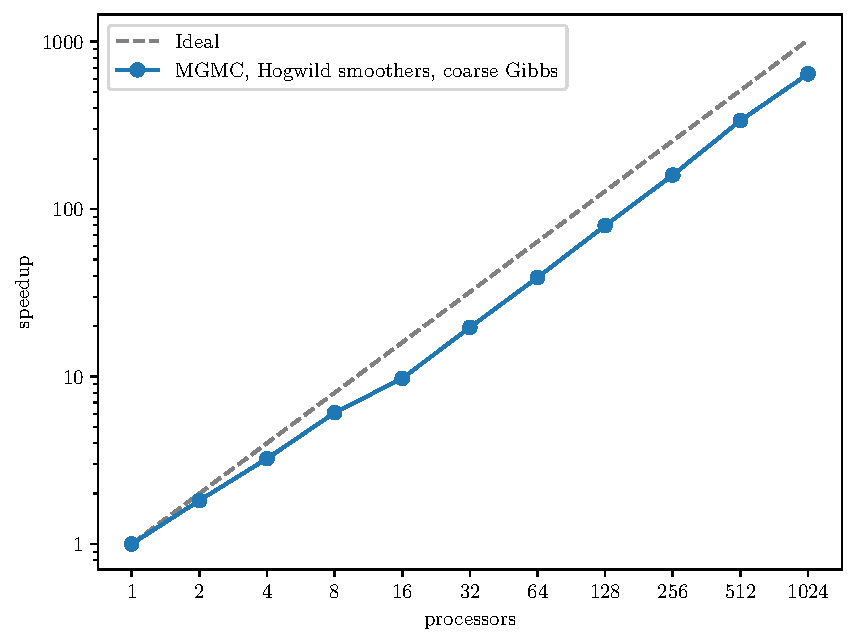
\includegraphics[width=\textwidth]{plots/strong_scaling_mgmc+hw+gibbs_4097x4097.pdf}
    \end{subfigure}
    \hfill
    \begin{subfigure}[b]{0.49\textwidth}
        \centering
        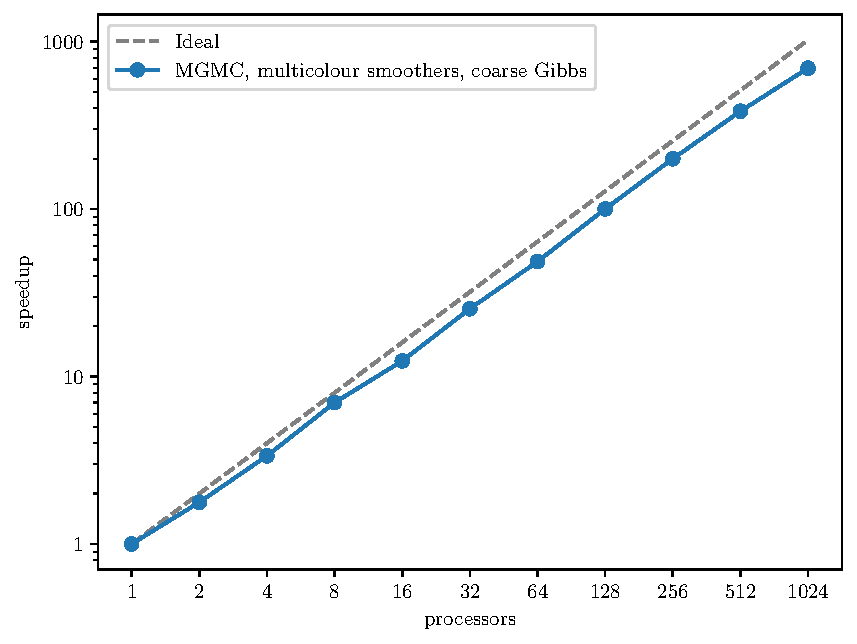
\includegraphics[width=\textwidth]{plots/strong_scaling_mgmc+mg+gibbs_4097x4097.pdf}
    \end{subfigure}
    \caption{Strong scaling speed-up for the MGMC sampler using Hogwild Gibbs as the random smoothers (left) and multicolour Gibbs as the random smoothers (right). Both use the respective variant of the Gibbs sampler also on the coarsest level.}
    \label{fig:2d_structured_mgmc_ss}
\end{figure}

The strong scaling behaviour changes if we use a Cholesky sampler on the coarsest level, see Fig.~\ref{fig:2d_structured_mgmc_chol_ss}. For this example we only considered MGMC with multicolour Gibbs random smoothers. We see that the performance deteriorates for more than 64 cores and the total runtime on 1024 processors is almost the same as for 128 processors. It should be noted that the Intel MKL Cholesky implementation offers some additional configuration options that could improve the performance (e.g., thread parallelisation within a processor) but we did not test the effect of these options yet.

\begin{figure}[htbp]
    \centering
    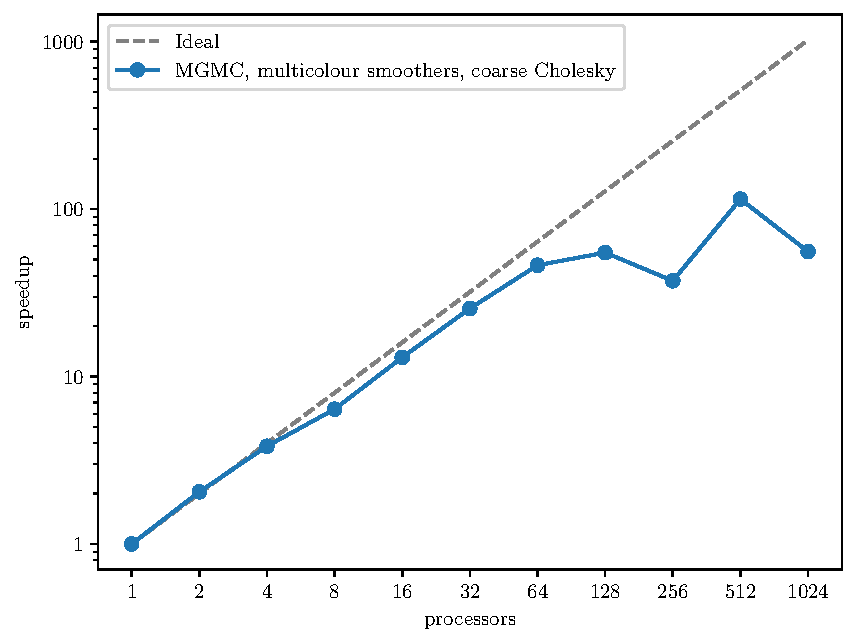
\includegraphics[width=0.7\textwidth]{plots/strong_scaling_mgmc+mg+cholesky_4097x4097.pdf}
    \caption{Strong scaling speed-up for the MGMC sampler using multicolour Gibbs as the random smoothers and Cholesky sampling on the coarsest level.}
    \label{fig:2d_structured_mgmc_chol_ss}
\end{figure}

\begin{table}[htpb]
    \centering
    \begin{tabular}{rccccc}
    \toprule
    \# Proc. & Fig.\ref{fig:2d_structured_ss} (right) & Fig.\ref{fig:2d_structured_ss} (left)  & Fig.\ref{fig:2d_structured_mgmc_ss} (right) & Fig.\ref{fig:2d_structured_mgmc_ss} (left) & Fig.\ref{fig:2d_structured_mgmc_chol_ss} \\
    \midrule
    {2}     &  94\% &  95\% &  89\% &  91\% & 102\% \\
    {4}     &  90\% &  87\% &  84\% &  81\% &  96\% \\
    {8}     &  86\% &  78\% &  87\% &  76\% &  80\% \\
    {16}    &  80\% &  75\% &  78\% &  61\% &  81\% \\
    {32}    &  89\% &  75\% &  79\% &  61\% &  80\% \\
    {64}    &  86\% &  80\% &  76\% &  61\% &  72\% \\
    {128}   &  86\% &  87\% &  78\% &  62\% &  43\% \\
    {256}   &  86\% &  95\% &  78\% &  62\% &  15\% \\
    {512}   &  82\% &  81\% &  75\% &  66\% &  22\% \\
    {1024}  &  68\% &  74\% &  68\% &  63\% &   5\% \\
    \bottomrule
    \end{tabular}
    \caption{Strong scaling efficiency for the 2D structured grid example.
      % ``Multicolour'' is abbreviated ``MC'', and ``Hogwild'' is abbreviated ``HW''. By MGMC+XX we mean that the Multigrid Monte Carlo sampler was used with ``XX Gibbs'' as the random smoother.
    }\label{tab:2d_structured_ss}
\end{table}

To conclude this example, we look at the weak scaling behaviour of the MGMC sampler. Fig.~\ref{fig:2d_structured_ws} shows the weak scaling efficiency for the multicolour Gibbs sampler, the MGMC sampler with Gibbs sweeps on the coarsest level, and MGMC using a coarse Cholesky sampler. The random smoother is a multicolour Gibbs sampler in both cases. We have fixed the local problem size of the coarsest level to $64 \times 64$ for all runs.

\begin{figure}[htbp]
    \centering
    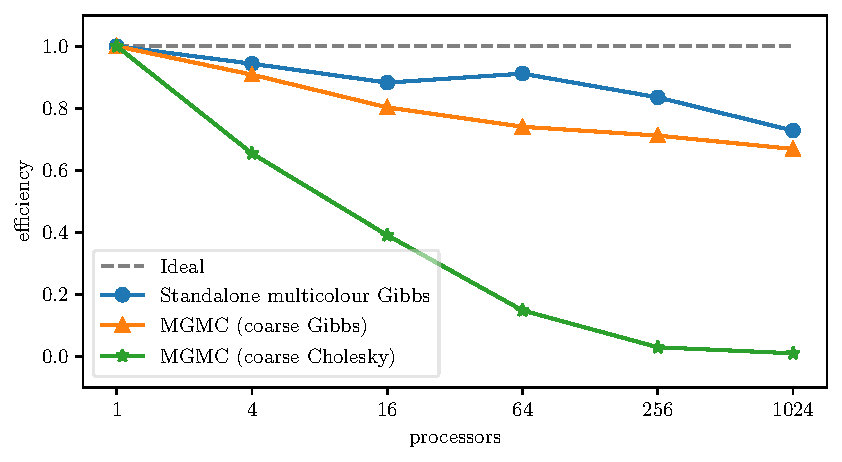
\includegraphics[width=0.8\textwidth]{plots/weak_scaling_64x64.pdf}
    \caption{Weak scaling efficiency for the multicolour Gibbs sampler and the MGMC sampler, using both Gibbs sampling and Cholesky sampling on the coarsest level. The random smoother is a multicolour Gibbs sampler in both cases.}
    \label{fig:2d_structured_ws}
\end{figure}

While both the standalone Gibbs sampler and the MGMC sampler with coarse Gibbs sampling show acceptable weak scaling performance, the use of the Cholesky sampler on the coarsest level seems to drastically reduce the efficiency. We note here again that this behaviour could be mitigated by adjusting the parameters in the Intel MKL library.

\subsection{Unstructured Grids}
In this section we consider two examples that discretise~\eqref{eq:shiftedlaplace} on unstructured grids using finite elements. The two grids are shown in Fig.~\ref{fig:mfem_ex}.

\begin{figure}[htbp]
    \centering
    \begin{subfigure}[b]{0.49\textwidth}
        \centering
        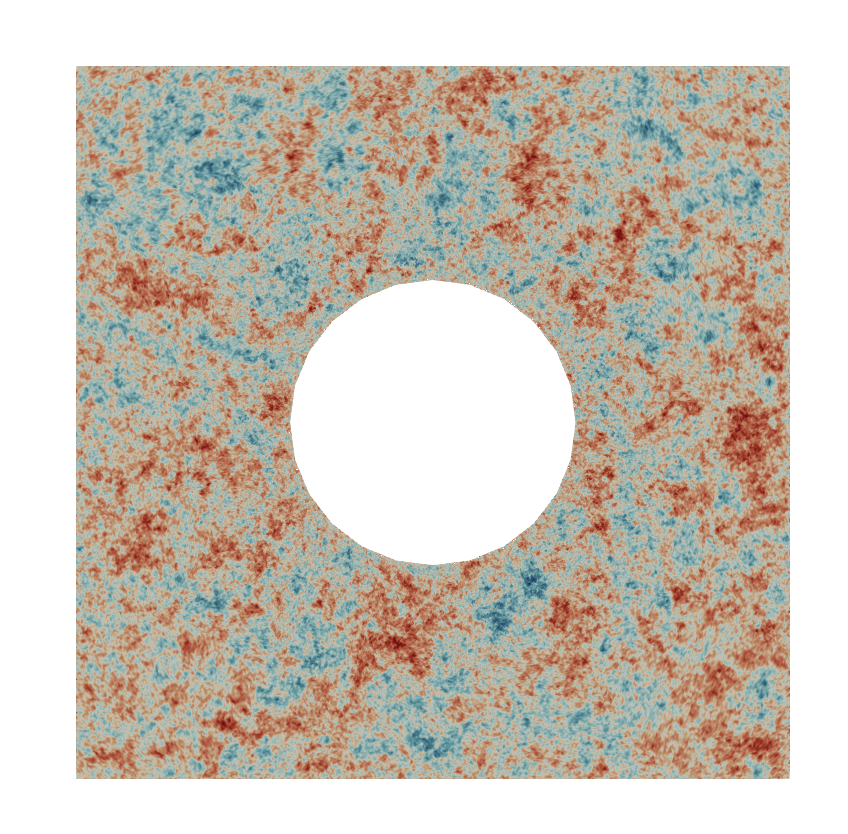
\includegraphics[width=\textwidth]{plots/paraview/square-disc_0_05.png}
    \end{subfigure}
    \hfill
    \begin{subfigure}[b]{0.49\textwidth}
        \centering
        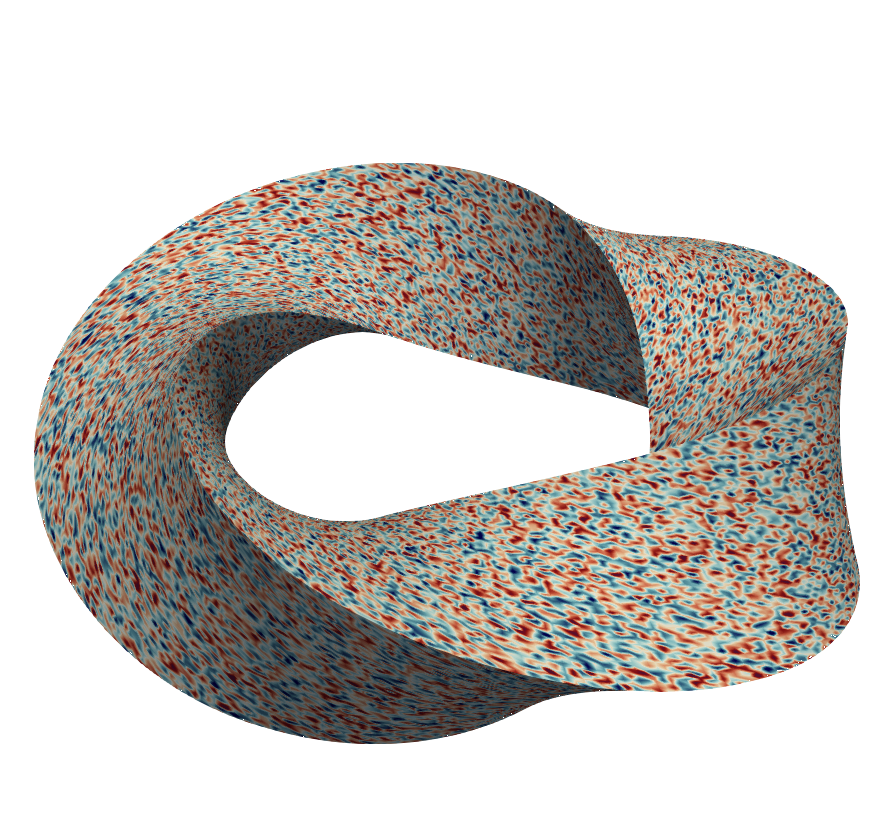
\includegraphics[width=\textwidth]{plots/paraview/toroid_1.png}
      \end{subfigure}
      \caption{Random samples on the grids discretised using finite elements. Both have precision operator $\kappa^2 - \Delta $, the square disc (left) uses $\kappa^{-1} = 0.05$, the twisted toroid (right) uses $\kappa^{-1} = 1$.}
    \label{fig:mfem_ex}
\end{figure}

We begin with a weak scaling test for the square disc example. In this case, instead of fixing the number of grids in the hierarchy, as well as the local coarse grid size, we fix the global coarse grid size and increase the number of levels with increasing number of cores. The number of levels ranges from three (for the one processor run) up to eight (for the run on 1024 processes). On the coarse grid we have $79616$ unknowns, on the finest grid there are approximately $1.2 \times 10^9$.

The number of colours required for the matrix colouring are (from coarse to fine)
\begin{equation*}
  7,\ 15,\ 18,\ 19,\ 19,\ 20,\ 20,\ 19\,.
\end{equation*}
These numbers differ slightly depending on the number of processors.

A plot of the weak scaling efficiency for the square disc example is given in Fig.~\ref{fig:2d_unstructured_ws}. We observe that neither sampler scales optimally, in particular when comparing the behaviour on four and sixteen cores to the single processor run. We also observe that unlike in the previous section, using a Cholesky sampler on the coarsest level does not affect the weak scaling performance much, indicating that the additional communication due to the colouring dominates the cost. Comparing absolute timings shows that the costs per sample of both variants of the MGMC sampler with multicolour Gibbs sweeps as random smoothers are within 10\% of each other for up to 64 processes; after that the coarse Cholesky sampler becomes more expensive.

\begin{figure}[htbp]
    \centering
    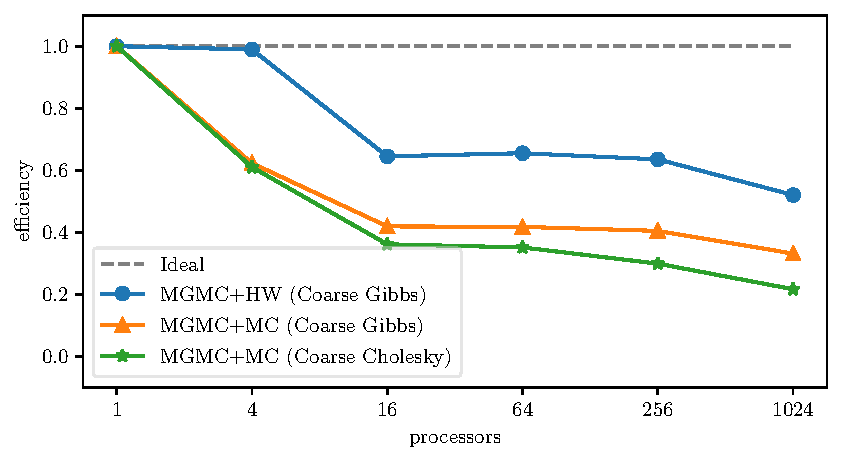
\includegraphics[width=0.7\textwidth]{plots/ws_mgmc_fe.pdf}
    \caption{Weak scaling efficiency for the  MGMC sampler applied to the square disc example.}
    \label{fig:2d_unstructured_ws}
\end{figure}

We continue to explore the effect of the coarse grid samplers by performing a strong scaling test for the toroid example. The grid hierarchy now consists of five levels (ranging from $2{\small,}160$ to $6{\small,}439{\small,}680$ unknowns) and the number of colours required to colour the matrix graphs are (from coarse to fine)
\begin{equation*}
  16,\ 45,\ 59,\ 63\,.
\end{equation*}
Again, these values depend on the number of processors that are used (the run with 1024 processes, for instance, required $16,47,61$ and $72$ colours, respectively). 

\begin{figure}[htbp]
    \centering
    \begin{subfigure}[b]{0.49\textwidth}
        \centering
        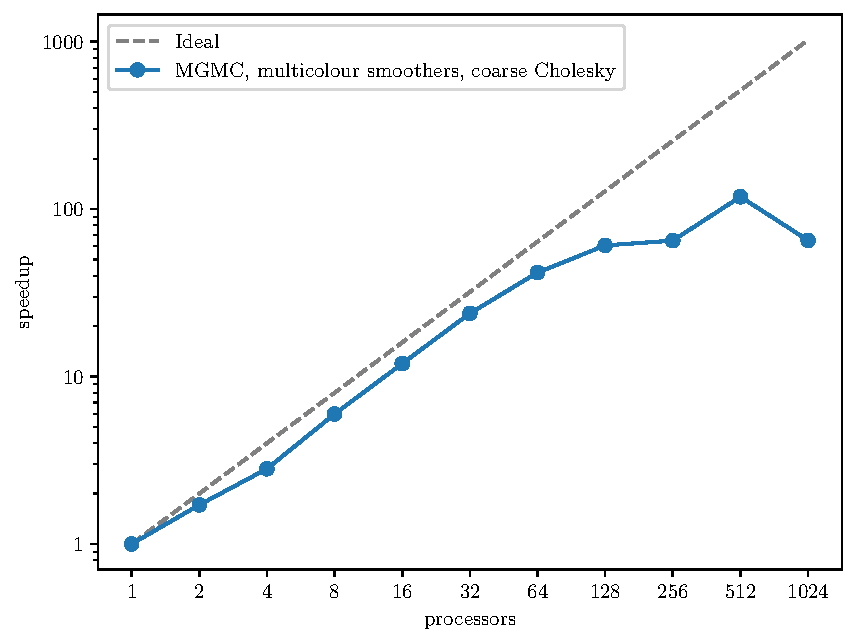
\includegraphics[width=\textwidth]{plots/strong_scaling_mgmc+mg+cholesky_toroid.pdf}
    \end{subfigure}
    \hfill
    \begin{subfigure}[b]{0.49\textwidth}
        \centering
        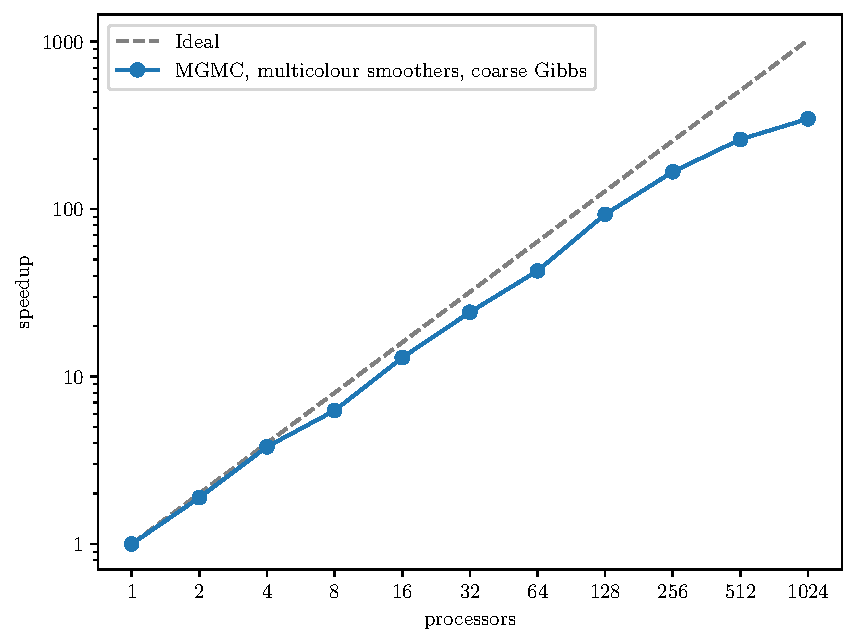
\includegraphics[width=\textwidth]{plots/strong_scaling_mgmc+mg+gibbs_toroid.pdf}
      \end{subfigure}
      \caption{Strong scaling speed-up for the toroid example. On the left, we used the MGMC sampler with Cholesky sampling on the coarsest grid, the right plot shows the results for using a multicolour Gibbs sampler instead. The random smoothers on the remaining levels are multicolour Gibbs samplers in both cases.}
    \label{fig:toroid_ss}
\end{figure}

The results are shown in Fig.~\ref{fig:toroid_ss}. Here, we again observe that the variant that uses a Cholesky sampler on the coarsest level scales worse than the sampler that uses multicolour Gibbs sweeps on the coarsest level. We also observe that the high number of colours on the coarser levels still allow for acceptable scaling, at least up to around 128 cores. Finally, we compare the absolute timings for this example. In Fig~\ref{fig:timings} we plotted the runtime for the two variants of the MGMC sampler. We report the time to set up the sampler and the time to generate 500 samples separately (the time to set up the finite element mesh hierarchy using the MFEM library is not included). We see that both sampler variants perform very similar up to 64 processes; after that, the sampling time for the Cholesky sampler stays approximately constant.

\begin{figure}[htbp]
    \centering
    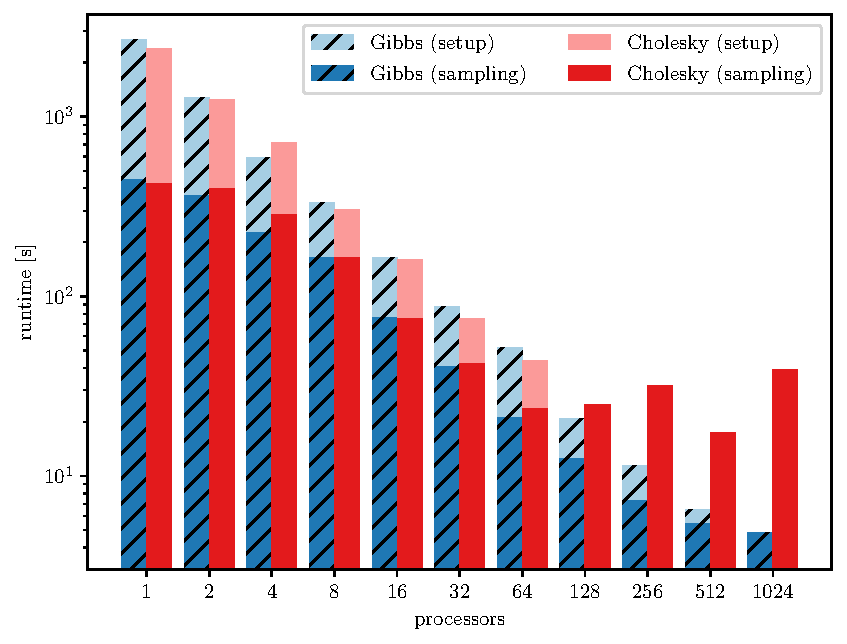
\includegraphics[width=0.7\textwidth]{plots/runtime.pdf}
    \caption{Comparison of the timings for the strong scaling example on the toroid mesh. The timings to set up the MGMC sampler and to generate the samples are reported separately. The left bars show the timings for the variant using a Gibbs sampler on the coarsest level, the right bars show timings using a coarse Cholesky sampler.}
    \label{fig:timings}
\end{figure}

\section{Conclusion}
In this report we have presented a parallel implementation of the Multigrid Monte Carlo method in PETSc. We have given a brief theoretical introduction to the method and an overview of the parallel implementation of the individual components of the sampler.

We then presented three numerical examples to study the scaling properties of the implementation, with particular focus on the effect of the colouring and the difference between the two coarse sampler types. It was demonstrated that the implementation shows acceptable strong and weak scaling if a simple red/black colouring can be used on the finest level, and Gibbs sweeps are used on the coarsest level. Using a Cholesky sampler reduced the performance.

The examples posed on unstructured grids both showed worse scaling due to the higher number of colours that are necessary to colour the matrix graph. For the two-dimensional example, neither sampler variant showed good weak scaling, and the performance was not affected much by using a coarse Cholesky sampler. For the three-dimensional example, we observed similar runtimes and strong scaling behaviour on up to $\sim 128$ processors; after that, the sampling cost of the Cholesky sampler variant does not decrease with increasing number of processors.

We also saw that if the number of colours is sufficiently low, using a Cholesky sampler on the coarsest level adversely affects the scalability. As noted above, this could be improved by introducing thread-parallelism on the level of individual cores, but it is well-known that multigrid scalability generally suffers from the non-optimal algorithmic complexity of direct coarse solvers (or samplers, in our case). A common strategy to improve upon this issue is to reduce the number of processors that participate on the coarser levels (e.g., the finest level use $64$ processors, the next level $16$, and the coarsest only one). This is sometimes referred to as \emph{agglomeration} and is implemented in PETSc for some grid configurations~\cite{petsc-multigrid}, and we plan to implement this strategy in a future version.

As we have seen in the examples, the number of colours typically grows from the finest to the coarsest level. This is due to definition of the coarse-level matrices by Galerkin projection of the finer level matrix. In geometric multigrid, another option to define the coarse-level problems is to rediscretise the operator on each level. In the two-dimensional structured grid example, this would mean that a red/black colouring would suffice on all levels, which could potentially reduce the overhead due to the communication of the boundary nodes. However, the convergence theory of~\cite{kazashimuellerscheichl} currently does not cover the case of precision matrices obtained by rediscretisations, and it is not known if the theory can be extended in this regard.


% \section{Notes}




% \subsection{Cholesky sampling from Gaussian distributions with given precision matrix}
% Suppose we want to generate samples from the distribution $\pi = \mathcal{N}(A^{-1} f, A^{-1})$. Let $LL^T = A$ be a Cholesky decomposition of the precision matrix $A$. Samples from $\pi$ can then be generated as follows:
% \begin{enumerate}
%     \item Draw a sample $\xi \sim \mathcal{N}(0,I)$.
%     \item Forward-solve $L g = f$ for $g$.
%     \item Backward-solve $L^T x = \xi + g$.
%     \item Return the new sample $x$.
% \end{enumerate}
% Indeed, we then have $x = L^{-T} \xi + L^{-T} g = L^{-T} \xi + {(LL^T)}^{-1} f =  L^{-T} \xi + A^{-1} f$ and by the properties of the normal distribution it follows that $x \sim \mathcal{N}(A^{-1} f, L^{-T}L^{-1}) = \mathcal{N}(A^{-1} f, A^{-1})$ as claimed.

% \subsection{Finite Difference discretisation of the shifted Laplace problem}
% Consider the following PDE
% \begin{align*}
%     -u_{xx}(x,y) - u_{yy}(x,y) + \kappa^2 u(x,y) &= f \qquad \text{for $0 < x,y < 1$} \\
%     u(x,y) &= 0 \qquad \text{for $x = 0, x = 1, y = 0, y = 1$.}
% \end{align*}
% Using a classic 5-point stencil, we obtain the discrete equations
% \begin{equation*}
%     -\frac{1}{h^2}\left(
%         u_{i+1,j} + u_{i,j+1} - 4u_{i,j} + u_{i,j-1} + u_{i-1,j}
%     \right)
%     + \kappa^2 u_{i,j} = 0\,,
% \end{equation*}
% for $i,j = 1,\dotsc,n-1$ and (due to the Dirichlet boundary condition)
% \begin{equation*}
%     u_{0,j} = u_{i,0} = u_{n,j} = u_{i,n} = 0\,, \qquad\text{for $i,j = 0,\dotsc,n$.} 
% \end{equation*}

% \subsection*{Mat\'ern Covariance functions and shifted Laplace PDEs}
% Consider the stochastic partial differential equation
% \begin{equation*}
%     \tau {(\kappa^2 - \Delta)}^{\alpha / 2} u = \mathcal{W}
% \end{equation*}
% posed on the whole of $\mathbb{R}^d$. Whittle has shown that the stationary solutions of this SPDE have Mat\'ern covariance with $\nu = \alpha - d/2$. Using a close connection between those solutions and the inner product of an associated reproducing kernel Hilbert space, one can show that the corresponding precision operator is
% \begin{equation*}
%     \mathcal{A}_\alpha \coloneqq \tau^2 {(\kappa^2 - \Delta)}^\alpha\,,
% \end{equation*}
%see~\cite[Sec.\ 2.2]{lindgrenSPDEApproachGaussian2022}.

% \section{Using a Gauss-Seidel implementation to implement a Gibbs sampler}
% Say we have access to a (parallel or sequential) Gauss-Seidel solver to solve the linear system
% $Ax = f$. The iteration can be written in matrix form as 
% \begin{equation*}
%     x^{(k+1)} = -D^{-1} L x^{(k+1)} - D^{-1}L^T x^{(k)} + D^{-1} f\,,
% \end{equation*}
% where $A = L + D + L^T$ with $L$ being the strictly lower triangular part of $A$, and $D$ being its diagonal. Let us compare this with the matrix form of a Gibbs sampler for generating a sequence of Gaussian samples $y^{(0)}, y^{(1)},\dotsc \sim \mathcal{N}(A^{-1}f, A^{-1})$ which is given by
% \begin{equation*}
%     y^{(k+1)} = - D^{-1} L y^{(k+1)} - D^{-1} L^T y^{(k)} + D^{-1} c^{(k)}\,,
% \end{equation*}
% with $c^{(k)} \sim \mathcal{N}(f, D)$. Thus, a Gauss-Seidel solver can be turned into a Gibbs sampler by repeatedly applying one Gauss-Seidel iteration to the linear system $Ax = c^{(k)}$.

\printbibliography
\end{document}

%%% Local Variables: 
%%% TeX-command-extra-options: "-shell-escape"
%%% End:
